\usetikzlibrary{positioning, arrows.meta}

\chapter{Задачі машинного навчання}

\section{Що таке модель?}

Насправді, чітко поставити задачу сучасної теорії машинного навчання одним
визначенням дуже складно. Це пов'язано з тим, що підхід до розв'язку задачі дуже
залежить від того, що ми очікуємо від так званої \textit{моделі машинного
навчання}. Що ж ми розуміємо під терміном ``модель''?

Найчастіше, на вхід подається певний набір данних $\mathcal{D}$. Це можуть бути
картинки разом з маркуванням, що зображено. Можуть бути текстові данні, чисельні
данні, аудіо- або відео-записи, результати вимірювань на сенсорних пристроях,
тощо. Маючи цей набір даних, ми часто хочемо зрозуміти певні закономірності в
цих даних. Функцію, що бере певний вхід, що містить інформацію про об'єкт, і
повертає вихід, що містить закономірність, часто називаємий
\textit{передбаченням}, як раз і називають \textbf{моделлю}. Далі наведемо
кілька нетривільних прикладів з задач машинного навчання.

\begin{example}[Класифікація цифр]
	Будь-яке сіро-біле зображення $\boldsymbol{X}$ розміру $W \times H$ пікселів
	можна розглядати як матрицю $\boldsymbol{X} \in \mathbb{R}^{W \times H}$, де
	кожен елемент матриці $X_{i,j}$ --- це значення яскравості відповідного
	пікселя на позиції $(i,j)$ (наприклад, значення $0$ може позначати чорний
	колір, $1$ --- білий, а значення проміж --- степінь сірості)\footnote{Іноді
	таку множину явно записують як $[0,1]^{W \times H}$, щоб підкреслити, що
	значення нормалізовані на відрізок $[0,1]$. Тим не менш, використовуємо
	позначення $\mathbb{R}^{W \times H}$, оскільки оптимальна нормалізація
	данних залежить від обраної методології}. 
	
	Нехай нам наданий набір $\mathcal{D} =
	\{(\boldsymbol{X}_n,y_n)\}_{1 \leq n \leq N}$ --- пари
	``зображення-цифра'', де $y_n \in \{0,\dots,9\}$. Наша ціль ---
	побудувати так звану \textit{класифікаційну модель} $f: \mathbb{R}^{W \times
	H} \to \{0,\dots,9\}$, яка буде приймати на вхід зображення
	$\boldsymbol{X}$ та видавати цифру $f(\boldsymbol{X})$, що зображена.
	Приклад зображено на Рисунку~\ref{fig:digits} на базі набору данних MNIST
	\cite{mnist}.

	\begin{figure}
		\centering
		\begin{tikzpicture}
			% Define grid and spacing size
			\def\gridsize{3}
			\def\xspacing{4} % Horizontal spacing
			\def\yspacing{3} % Vertical spacing
			
			% Loop to create 3x3 grid with predictions
			\foreach \row in {1,2,3} {
				\foreach \col in {1,2,3} {
			
					% Calculate image index for sample prediction (0-9, can be random or set)
					\pgfmathtruncatemacro{\digitindex}{(\row-1)*\gridsize + \col - 1}

					% Placeholder integer predictions (customize as needed)
					\pgfmathtruncatemacro{\prediction}{mod(\digitindex, 10)} % Dummy prediction for illustration
					
					% Position of each MNIST image
					\node[draw, minimum size=1cm, inner sep=0pt] (img\row\col) at (\col*\xspacing, -\row*\yspacing)
					{\includegraphics[width=1.75cm]{figures/mnist/digit\digitindex.png}};
			
					% Prediction label with actual prediction value next to each digit
					\node[right=1.0cm of img\row\col] (pred\row\col) {\textbf{\prediction}};
			
					% Arrow pointing from image to prediction
					\draw[->, thick] (img\row\col) -- node[above] {\( f \)} (pred\row\col);
				}
			}
		\end{tikzpicture}
		\caption{Приклад класифікації цифр. Маючи зображення $X \in \mathbb{R}^{W \times H}$, наша функція дає дискретне передбачення $f(X) \in \{0,\dots,9\}$ --- цифра, яка зображена на зображенні $X$.}
		\label{fig:digits}
	\end{figure}

\end{example}

\begin{example}[Розпізнавання дрону]
	Нехай наша задача: це розпізнати розташування дронів на кадрі відео. Нехай в
	нас кольорове зображення розміру $W \times H$. Тоді зображення
	$\boldsymbol{X}$ береться з множини $\mathbb{R}^{W \times H \times 3}$,
	де замість яскравості пікселя, маємо тривимірний вектор $(r,g,b) \in
	\mathbb{R}^3$ --- колір пікселя (інтенсивність червоного, зеленого та синіх
	каналів, відповідно).

	Поділимо наше зображення на сітку розміру $n_W \times n_H$. Тоді в якості
	моделі можна взяти функцію $f: \mathbb{R}^{W \times H \times 3} \to
	\mathbb{R}^{n_W \times n_H}$, що видає матрицю
	$\{p(S_{i,j}|\boldsymbol{X})\}_{1 \leq i \leq n_W, \, 1 \leq j \leq n_H}$,
	де $S_{i,j}$ --- подія ``в клітинці $(i,j)$ сітки знаходиться дрон''. Ця
	модель візуально проілюстрована на Рис.~\ref{fig:drone}. Відмітимо, що ідея
	описаної конструкції частково використовується в архітектурі YOLO (You Look
	Only Once) \cite{yolo} --- одній з найпопулярніших архітектур для
	розпізнавання об'єктів на зображеннях.

	\begin{figure}
	
	\centering
	\begin{tikzpicture}

		% Set up background image
		\node[inner sep=0pt, anchor=center] at (0,0) {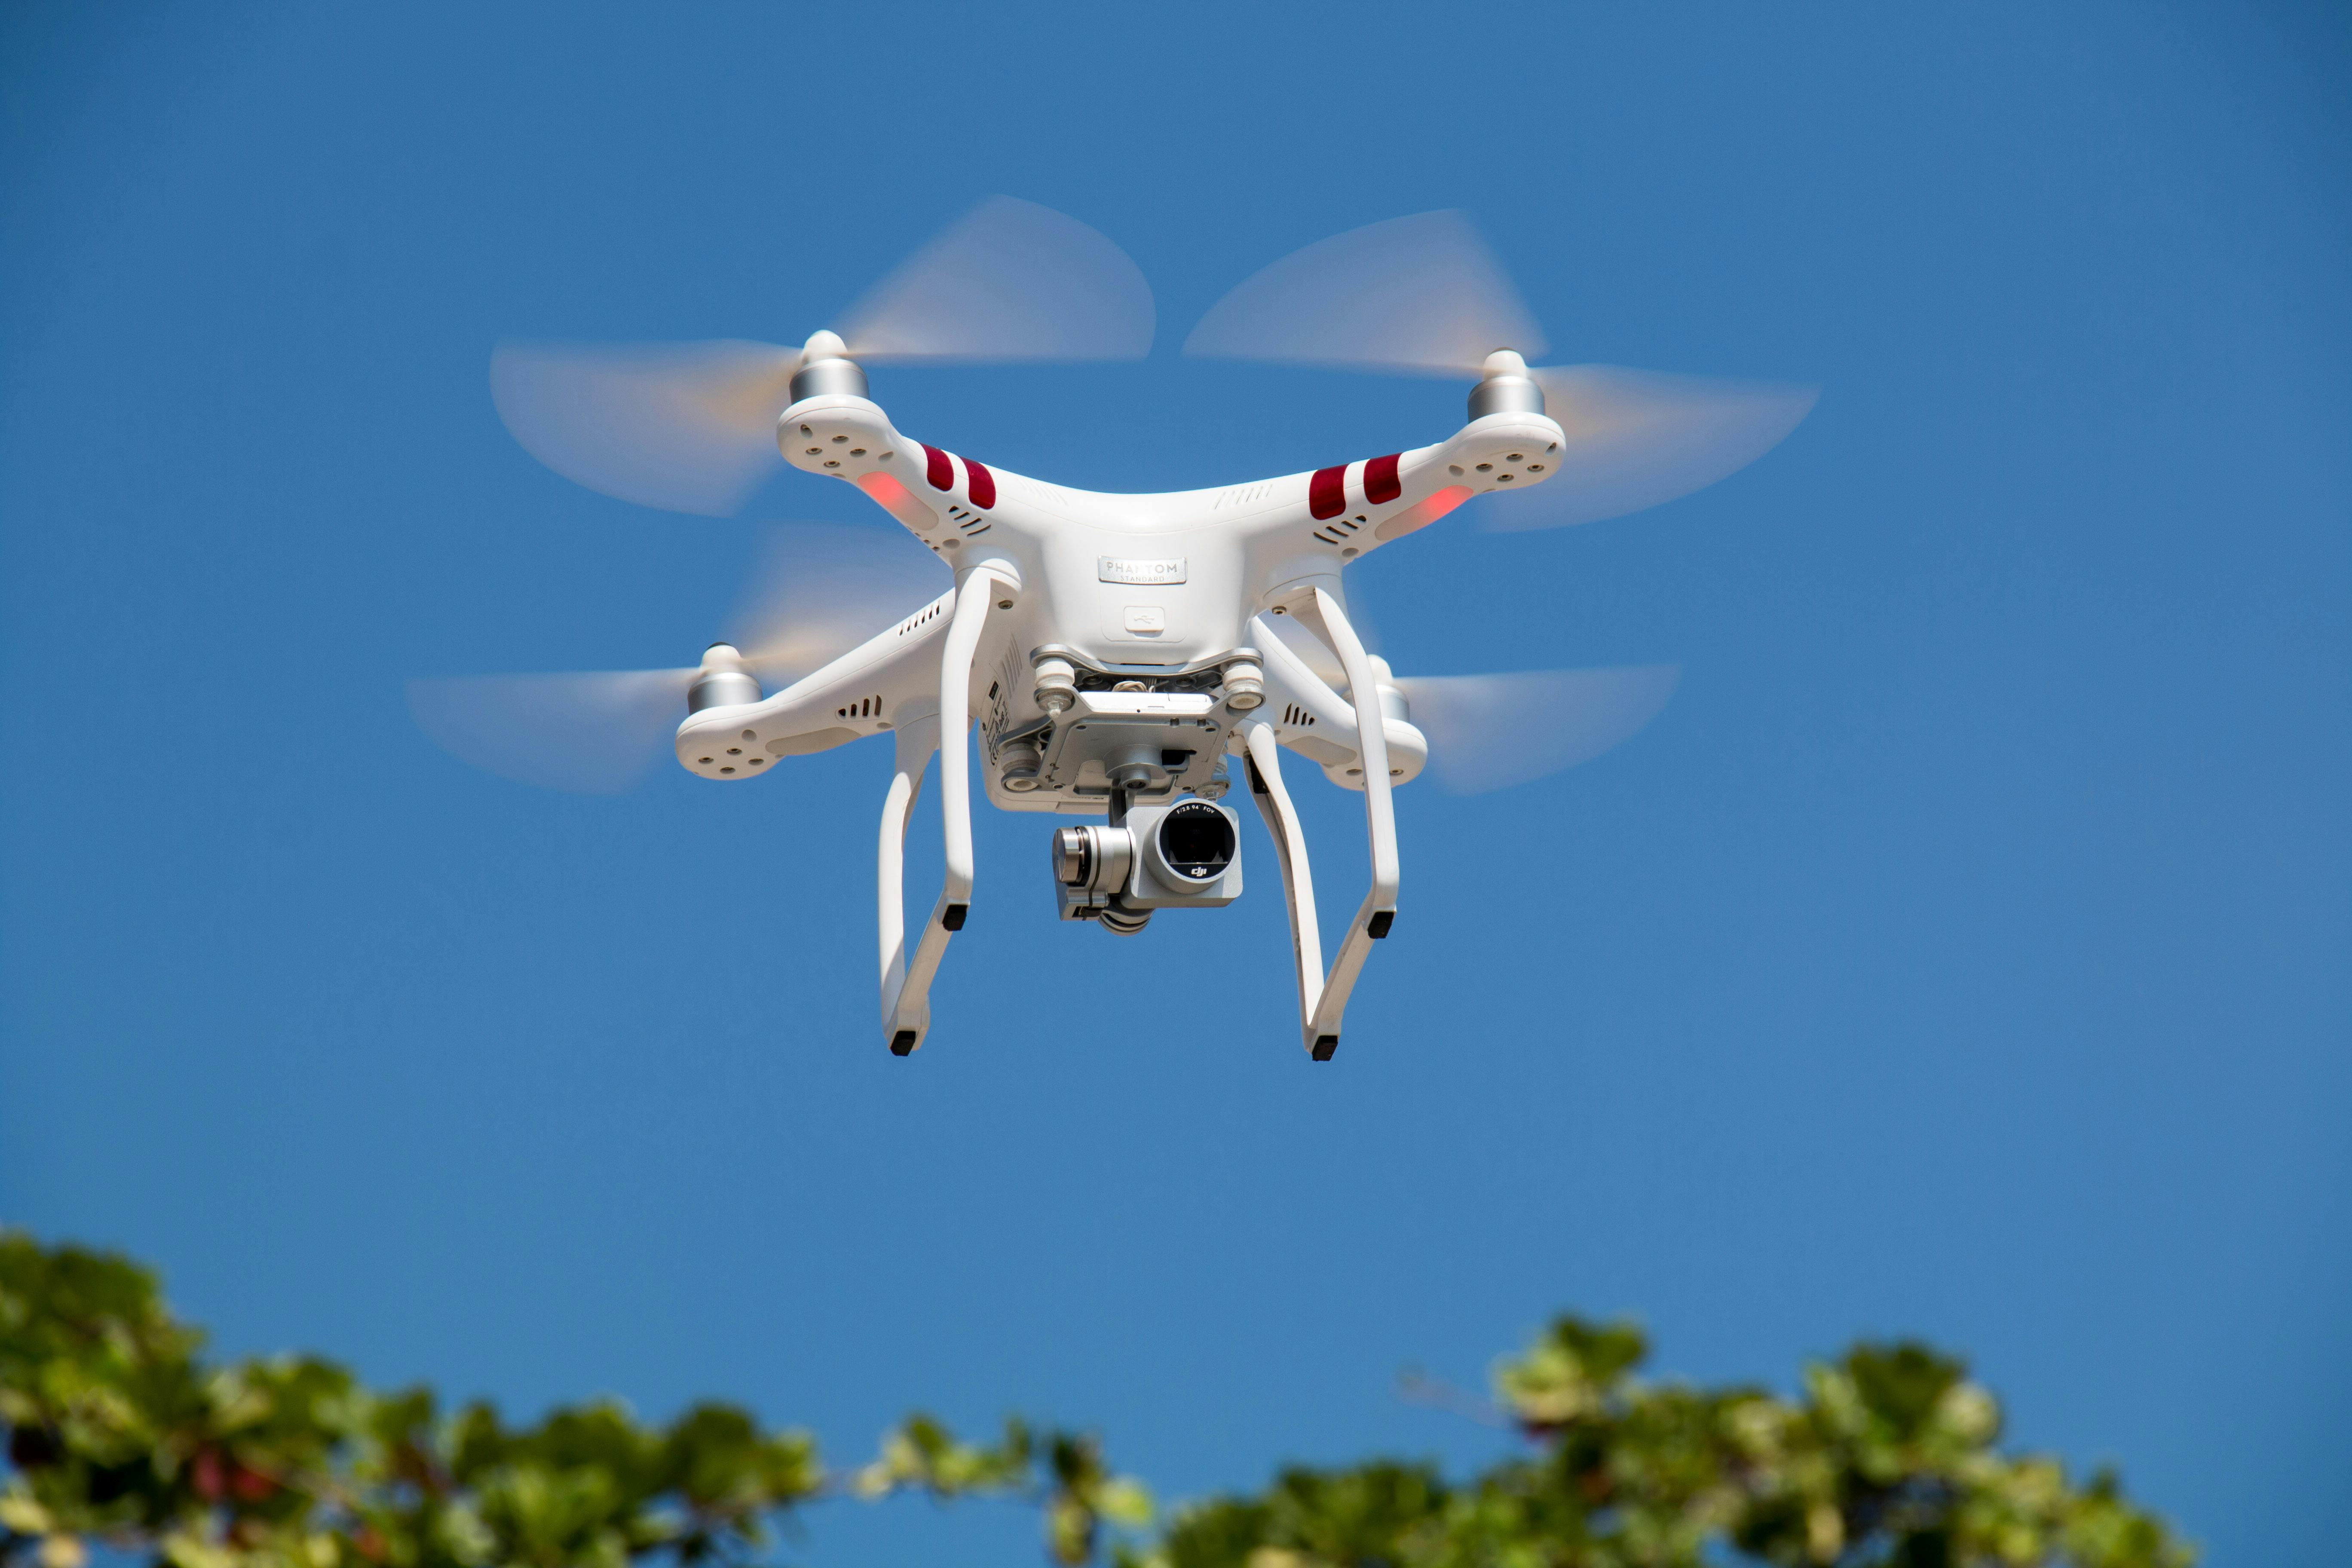
\includegraphics[width=10cm]{drone.jpg}}; % Replace 'background_image.jpg' with the path to your image
		
		% Define grid parameters
		\def\gridsize{7}
		\def\cellsize{1.5} % Size of each cell
		
		% Define the location of the object in the background (center of the image)
		\def\objectX{0} % X position of the object (centered in the image)
		\def\objectY{0} % Y position of the object (centered in the image)
		
		% Draw the gradient grid overlay with dashed borders
		\foreach \x in {-3,-2,-1,0,1,2} {
			\foreach \y in {-2,-1,0,1} {
				\definecolor{cellcolor}{rgb}{0.6, 0.8, 1} % Cold color (light blue)
				\ifnum\x=0\ifnum\y=0
					\definecolor{cellcolor}{rgb}{1, 0.6, 0.6} % Warm color (red/pink)
				\fi\fi
				\ifnum\x=-1\ifnum\y=0
					\definecolor{cellcolor}{rgb}{1, 0.6, 0.6} % Warm color (red/pink)
				\fi\fi
				\ifnum\x=-2\ifnum\y=0
					% Light yellow
					\definecolor{cellcolor}{rgb}{1, 1, 0.6}
				\fi\fi
				\ifnum\x=0\ifnum\y=-1
				\definecolor{cellcolor}{rgb}{1, 0.8, 0.4} % Intermediate warm (orange/yellow)
				\fi\fi
				\ifnum\x=-1\ifnum\y=-1
				\definecolor{cellcolor}{rgb}{1, 0.8, 0.4} % Intermediate warm (orange/yellow)
				\fi\fi

				% % Calculate distance from the object's location
				% \pgfmathsetmacro{\distance}{sqrt((\x - \objectX)^2 + (\y - \objectY)^2)}
		
				% % Set color based on distance to simulate probability heatmap
				% \ifdim \distance pt < 1.5pt
				% 	\definecolor{cellcolor}{rgb}{1, 0.6, 0.6} % Warm color (red/pink)
				% \else\ifdim \distance pt < 2.5pt
				% 	\definecolor{cellcolor}{rgb}{1, 0.8, 0.4} % Intermediate warm (orange/yellow)
				% \else
				% 	\definecolor{cellcolor}{rgb}{0.6, 0.8, 1} % Cold color (light blue)
				% \fi\fi
		
				% Overlay gradient cell with transparency
				\fill[cellcolor, opacity=0.5] (\x*\cellsize, \y*\cellsize) rectangle ++(\cellsize, \cellsize);
		
				% Draw dashed border around each cell
				\draw[line width=1pt, dashed] (\x*\cellsize, \y*\cellsize) rectangle ++(\cellsize, \cellsize);
			}
		}

		\draw[<-, ultra thick, bend right=90] (2.5,2) -- ++(3.0,-1) node[right] {$f_{1,5}(X) \approxeq 0.02$}; % Adjust coordinates for proper alignment
		\draw[<-, ultra thick, bend right=90] (0.5,-0.5) -- ++(6.0,-1) node[right] {$f_{3,4}(X) \approxeq 0.40$}; % Adjust coordinates for proper alignment

		\end{tikzpicture}
		\caption{Приклад розпізнавання дронів. Маючи зображення $\boldsymbol{X} \in \mathbb{R}^{W \times H \times 3}$, наша функція дає ймовірність того, що на кожному сегменті зображення знаходиться дрон. Чим тепліше кольори, тим вища ймовірність.}
		\label{fig:drone}
	\end{figure}
\end{example}

\begin{remark}
	Зверніть увагу, що в обох прикладах вище, модель $f$ видає дискретне або
	неперервне передбачення. Це може бути класифікація, регресія, сегментація,
	тощо. Це залежить від задачі, що ми розв'язуємо.
\end{remark}

\section{Параметризація моделей}
Проте, як саме ми будуємо моделі? Іншими словами, як обрати функцію $f$?
Зазвичай, ми маємо задати певне сімейство функцій $\mathcal{F}$, поміж яких ми
шукаємо ``найкращу''\footnote{Що таке ``найкраща'' функція, ми обговоримо
пізніше.} функцію. Наприклад, це може бути сімейство лінійних/квадратичних
функцій або функцій вигляду $f(x) = (\theta_1x^2, \theta_2 x)$. Звичайно,
оскільки алгоритм пошуку $f$ має бути заданий програмно, то ми не можемо
покласти в якості $\mathcal{F}$, скажімо, просто $L^2(\mathbb{R})$, бо тоді не
зрозуміло, як саме задати алгоритм пошуку $f$. Саме тому, для практичних
застосувань, ми \textit{параметризуємо} функції набором параметрів
$\boldsymbol{\theta}\in \Theta \subset \mathbb{R}^m$. Таким чином, наша модель
має вигляд $f(\mathbf{x}|\boldsymbol{\theta})$, де параметри
$\boldsymbol{\theta}$ можна змінювати, щоб зробити модель точною.

\begin{example}[Лінійна Регресія]
	Одна з класичних та найбільш відомих моделей --- це лінійна регресія. Нехай
	маємо набір даних $\mathcal{D} = \{(\mathbf{x}_n, y_n)\}_{1 \leq n \leq N}
	\subset \mathbb{R}^m \times \mathbb{R}$ і ми вважаємо, що залежність між
	$\mathbf{x}_n$ та $y_n$ лінійна. Іншими словами, ми введемо модель
	$f(\mathbf{x}|\boldsymbol{\theta}) = \boldsymbol{w}^{\top} \mathbf{x} +
	\beta$, де $\boldsymbol{\theta}=(\boldsymbol{w},\beta) \in \mathbb{R}^{m+1}$
	--- вектор параметрів. 

	В цілому, саме так дуже часто вводиться модель лінійної регресії. Проте, часто
	в літературі можна зустріти у якості моделі \textit{розподіл} величини $y$:
	\begin{equation}
		p(y|\mathbf{x},\boldsymbol{\theta}) = \mathcal{N}(y|\boldsymbol{w}^{\top}\mathbf{x} + \beta, \sigma^2),
	\end{equation}
	де $\boldsymbol{\theta} = (\boldsymbol{w},\beta,\sigma^2)$ --- вектор
	параметрів, а $\mathcal{N}(y|\mu,\sigma^2)$ --- щільність нормального
	розподілу. Така альтернатива дозволяє ввести більш гнучку модель, яка може
	давати степінь впевненості у своїх передбаченнях.
\end{example}

\begin{remark}
	Приклад вище легко узагальнити для випадку, коли вихід $\mathbf{y} \in \mathbb{R}^r$ --- вектор. В такому випадку, 
	моделлю є передбачення наступного розподілу:
	\begin{equation}
		p(\mathbf{y}|\mathbf{x},\boldsymbol{\theta}) = \prod_{i=1}^r \mathcal{N}(y_i|\boldsymbol{w}_i^{\top}\mathbf{x} + \beta_i, \sigma_i^2), \; \boldsymbol{w}_i \in \mathbb{R}^m, \; \beta_i,\sigma_i \in \mathbb{R}
	\end{equation}
\end{remark}

Отже, нехай ми вибрали параметризацію моделі. Як тепер обрати найкращі параметри?
Тут, наскільки б це не звучало банально, але знову все залежить від того, що ми
очікуємо від моделі:
\begin{itemize}
	\item Якщо наша модель має апроксимувати певну функцію $\varphi(\mathbf{x})$ на 
	обмеженій множині $\mathcal{X} \subset \mathbb{R}^r$, то ми можливо хочемо 
	мінімізувати $L^2(\mathcal{X},\mu)$ норму різниці:
	\begin{equation*}
		\widehat{\boldsymbol{\theta}} = \argmin_{\boldsymbol{\theta} \in \Theta} \int_{\mathcal{X}} d\mu(\mathbf{x}) \left\| f(\mathbf{x}|\boldsymbol{\theta}) - \varphi(\mathbf{x}) \right\|_2^2
	\end{equation*}
	\item Можливо, ми хочемо максимізувати функцію правдоподібності:
	\begin{equation*}
		\widehat{\boldsymbol{\theta}} = \argmax_{\boldsymbol{\theta} \in \Theta} \prod_{n=1}^N p(y_n|\mathbf{x}_n,\boldsymbol{\theta})
	\end{equation*}
	\item Якщо модель видає ймовірністний розподіл над простором $\Omega \subset \mathbb{R}^r$, то можливо ми хочемо мінімізувати відстань Кульбака-Лейблера до заданого розподілу $\pi(\mathbf{x})$:
	\begin{equation*}
		\widehat{\boldsymbol{\theta}} = \argmin_{\boldsymbol{\theta} \in \Theta} D_{\mathbb{KL}}(f(\mathbf{x}|\boldsymbol{\theta})||\pi(\mathbf{x})) = \argmin_{\boldsymbol{\theta} \in \Theta} \int_{\Omega} f(\mathbf{x} | \boldsymbol{\theta}) \log \frac{f(\mathbf{x} | \boldsymbol{\theta})}{\pi(\mathbf{x})}d\mathbf{x}
	\end{equation*}
\end{itemize}

\begin{example}[Розв'язок лінійної регресії]
	Наприклад, нехай ми вирішуємо задачу лінійної регресії для набору даних
	$\mathcal{D} = \{(\mathbf{x}_n, y_n)\}_{1 \leq n \leq N}$. Нехай ми хочемо 
	мінімізовувати функцію правдоподібності:
	\begin{equation}
		\widehat{\boldsymbol{\theta}} = \argmax_{\boldsymbol{\theta} \in \Theta} \prod_{n=1}^N p(y_n|\mathbf{x}_n,\boldsymbol{\theta}) = \argmax_{(\boldsymbol{w},\beta,\sigma^2)}\prod_{n=1}^N \mathcal{N}(y_n|\boldsymbol{w}^{\top}\mathbf{x}_n+\beta,\sigma^2)
	\end{equation}

	Можна довести, що якщо позначити $\mathbf{X} = [\mathbf{x}_1,\dots,\mathbf{x}_N] \in \mathbb{R}^{m \times N}$ --- матриця даних, а $\mathbf{y} = [y_1,\dots,y_N] \in \mathbb{R}^N$ --- вектор маркерів, то розв'язок має вигляд:
	\begin{equation}
		\widehat{\boldsymbol{\theta}} = (\mathbf{X}\mathbf{X}^{\top})^{-1}\mathbf{X}\mathbf{y}
	\end{equation}
\end{example}

Проте, яку б ми теорію не використовували і які б параметризації моделей не
використовували, в кінці кінців, перед нами постає наступна задача оптимізації, що
розв'язується чисельно:
\begin{equation}
	\widehat{\boldsymbol{\theta}} = \argmin_{\boldsymbol{\theta} \in \Theta} \mathcal{L}(\mathcal{D}|\boldsymbol{\theta}),
\end{equation}

де $\mathcal{L}(\mathcal{D}|\boldsymbol{\theta})$ --- функція втрат, яка
відображає як добре модель з параметрами $\boldsymbol{\theta}$ апроксимує дані
$\mathcal{D}$. Зауважимо, що хоч, в ідеалі, ми хочемо отримати вихід як
найближчий до ``істинного'', але в більшості випадків, ми не знаємо
``істинного'' вихідного розподілу. Тому, функція втрати, на практиці, 
залежить від набору данних $\mathcal{D}$, що подається на вхід, та від
параметризації $\boldsymbol{\theta}$.

Отже, стає питання: а як обрати параметризацію? Насправді, саме в цьому питанні
лежить більшість сучасних досліджень у глибокому навчанні: наприклад, у 1995
році, конволюційні нейронні мережі (Convolutional Neural Networks --- CNN)
прийшли на заміну повнозв'язним нейронним мережам \cite{lecun}, а механізм уваги
(Attention) у 2017 став основою багатьох NLP нейронних мереж \cite{attention}.
Щоб підкреслити важливість цього питання, наведемо приклад.

\begin{example}
	Нехай ми хочемо апроксимувати залежність $y(x)$ для набору $\mathcal{D} =
	\{(x_n,y_n)\}_{1 \leq n \leq N}$, причому навіть знаючи вибірку, ми не маємо
	уяви, яка має бути залежність $y(x)$. За невідомими причинами, нехай ми
	вирішили використати модель $f(x|\boldsymbol{\theta}) =
	\left(\sum_{i=1}^{1000}\theta_i\right)x$ для вектору параметрів
	$\boldsymbol{\theta} \in \mathbb{R}^{1000}$. Хоча ця модель містить досить
	велику кількість параметрів, вона не може апроксимувати жодні залежності
	окрім лінійних. Отже навіть якщо залежність $y$ від $x$ квадратична, що
	є відносно простою залежністю, модель не зможе її апроксимувати, незважаючи 
	на велику кількість параметрів.
\end{example}

\section{Основні задачі машинного навчання}

Отже, на практиці, ми хочемо мати як можна меньше параметрів, але при цьому 
модель повинна бути достатньо гнучкою, щоб апроксимувати будь-яку залежність. 
Інакшими слвоами, модель має апроксимувати як можна більш широкий клас 
функцій. 

Таким чином, підсумуємо, перед якими проблемами стоїть дослідник у глибокому
навчанні. Ми виділили три основні проблеми, які можна сформулювати наступним
чином: 
\begin{enumerate}
	\item \textbf{Проблема статистики/ймовірності/узагальнення:} маючи лише
	набір данних $\mathcal{D}$, не знаючи істинного розподілу чи функції, чи
	достатньо добре функція втрати $\mathcal{L}$ відображає степінь наближення
	моделі до істинної функції або розподілу?
	\item \textbf{Проблема оптимізації:} маючи функцію втрати $\mathcal{L}$,
	наскільки точно і чи взагалі можливо знайти оптимальні параметри
	$\boldsymbol{\theta}$ для мінімізації функції втрати?
	\item \textbf{Проблема апроксимації:} яка найкраща і чи взагалі існує така
	параметризація моделі, щоб вона була достатньо гнучкою, але при цьому мала
	якнайменшу кількість параметрів?\footnote{Мала кількість параметрів сприяє
	як і, очевидно, швидкості навчання та діставання передбачень, так і робить
	модель менш схильною до перенавчання та проблем градієнтів (стосується
	проблеми оптимізації).}
\end{enumerate}

В наступному підрозділі, ми розглянемо декілька теорем, що 
дозволяють відповісти на третє запитання. Після цього, ми перейдемо 
до методології другої проблеми, а саме, до методів оптимізації.
